\documentclass[12pt]{article}
 \usepackage[margin=1in]{geometry} 
\usepackage{amsmath,amsthm,amssymb,amsfonts}
\usepackage{graphicx}

\newcommand{\N}{\mathbb{N}}
\newcommand{\Z}{\mathbb{Z}}
 
\newenvironment{problem}[2][]{\begin{trivlist}
\item[\hskip \labelsep {\bfseries #1}\hskip \labelsep {\bfseries #2.}]}{\end{trivlist}}

\begin{document}
  
\title{Computational Physics Project 2: Time Independent Schrodinger Equation}
\author{Ben Zager, Christopher Meierfrankenfeld}
\maketitle
 
\section*{Solving the TISE}

\begin{figure}[ht!]
	\centering
	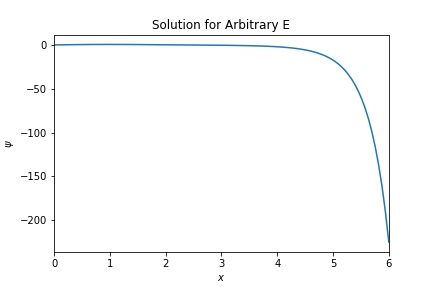
\includegraphics[scale=0.6]{../figures/guessPlot_L=6_E=2.png}
	\caption{Solution to TISE using and arbitrary guess of $E=2$}
	\label{guess}
\end{figure}

\section*{Root Finding}

\begin{figure}[ht!]
	\centering
	\begin{minipage}[b]{0.4\textwidth}
		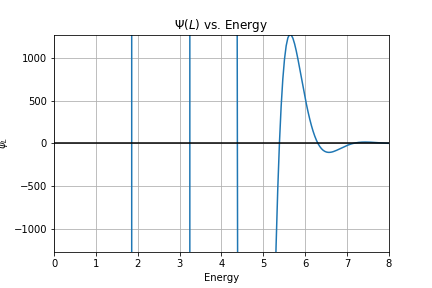
\includegraphics[scale=0.6]{../figures/psiAtL_EMax=8.png}
	\end{minipage}
	\hfill
	\begin{minipage}[b]{-- 0.4\textwidth}
		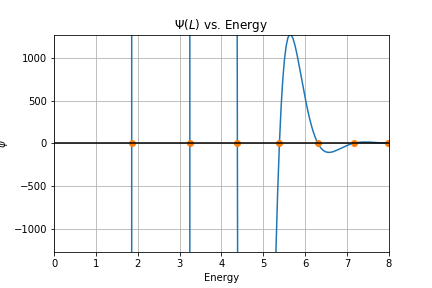
\includegraphics[scale=0.6]{../figures/rootsFound.png}
	\end{minipage}
	\caption{Solution at L as function of energy.  Original plot is shown on left, and plot after finding roots is shown on right.}
	\label{root}
\end{figure}

\section*{Normalization}

\begin{figure}[ht!]
	\centering
	\begin{minipage}[b]{0.4\textwidth}
		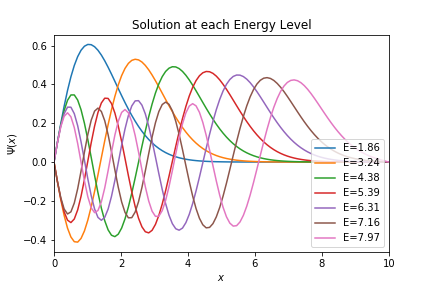
\includegraphics[scale=0.6]{../figures/wavefunctions.png}
	\end{minipage}
	\hfill
	\begin{minipage}[b]{-- 0.4\textwidth}
		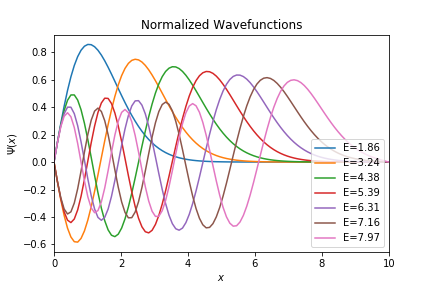
\includegraphics[scale=0.6]{../figures/normalized.png}
	\end{minipage}
	\caption{}
	\label{psi}
\end{figure}

\section*{Analytical Solution}

\begin{figure}[ht!]
	\centering
	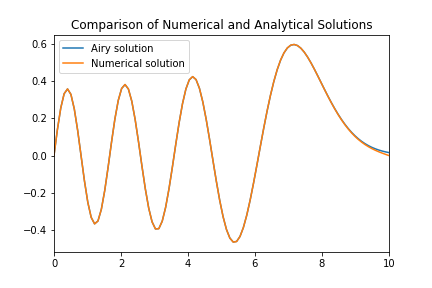
\includegraphics[scale=0.6]{../figures/airy_n=7.png}
	\caption{Numerical solution plotted with Airy function solution for $n=7$}
	\label{airy}
\end{figure}

\end{document}
